\documentclass[12pt,a4paper]{report}
\usepackage[utf8]{inputenc}
\usepackage[english,russian]{babel}
\usepackage{indentfirst}
\usepackage{pdfpages}
\usepackage{titlesec}
\usepackage{listings}
\usepackage{amsmath}

% Вставка картинки
\usepackage{graphicx}
\graphicspath{{schemes/}}
\DeclareGraphicsExtensions{.pdf,.png,.jpg}

\usepackage[14pt]{extsizes}

\newcommand{\hsp}{\hspace{20pt}}
\titleformat{\chapter}[hang]{\large\bfseries}{\thechapter{. }}{0pt}{\large\bfseries}
\titlelabel{hlabel-formati}
\titlespacing{\chapter}{42pt}{-20pt}{12pt}
\titleformat{\section}[hang]{\large\bfseries}{\thesection{. }}{0pt}{\large\bfseries}
\titlespacing{\section}{42pt}{12pt}{5pt plus 5pt}

% Отступ абзаца
\usepackage{indentfirst}
\setlength{\parindent}{1.5cm}

% Межстрочный интервал
\usepackage{setspace}
\onehalfspacing % интервал 1.5

\usepackage[left=3cm, right=1cm, top=2cm, bottom=2cm]{geometry}

\begin{document}
% Титульник
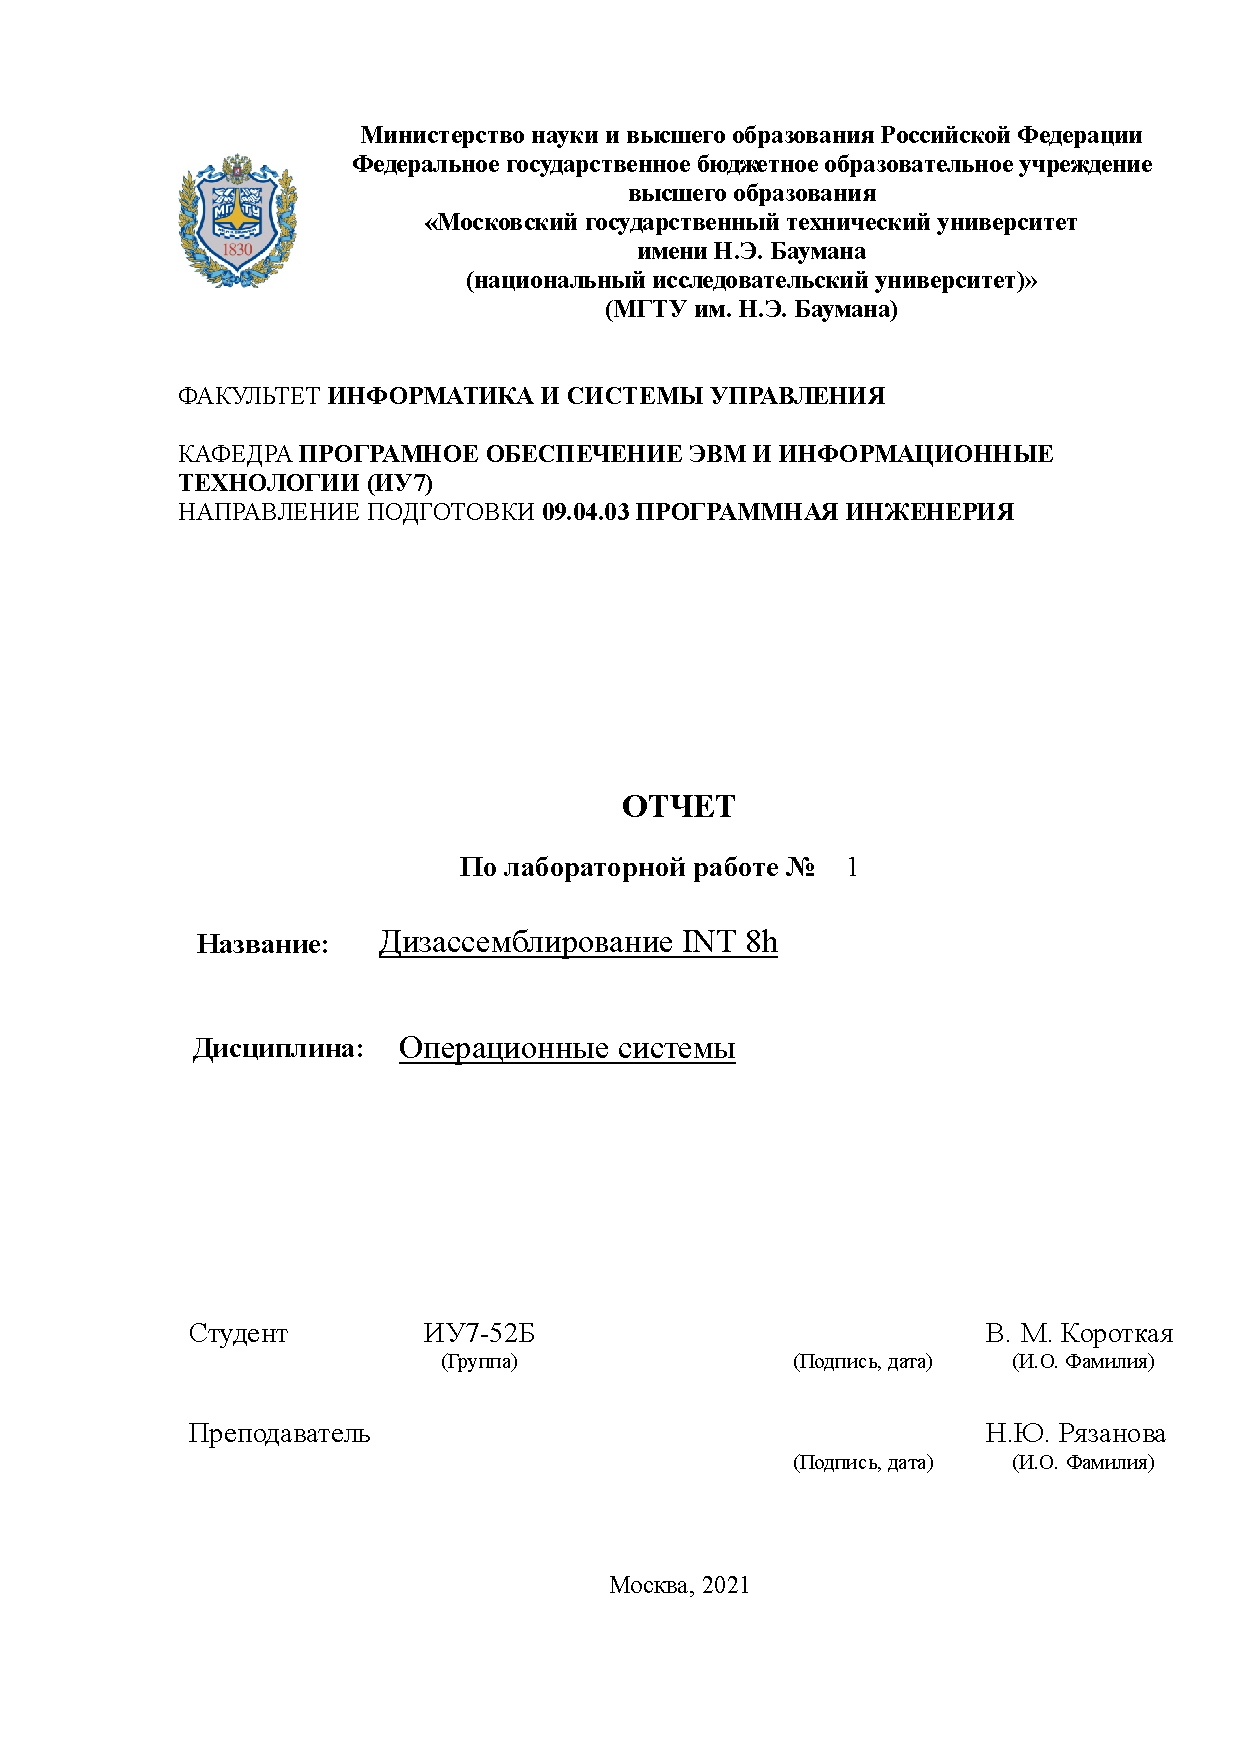
\includepdf[pages=1]{titul.pdf}

\begin{lstlisting}[label=some-code,caption=Код прерывания INT 8h]
    ; Вызывает подпрограмму sub_1
    020A:0746  E8 0070		;*		call	sub_1			; (07B9)
    020A:0746  E8 70 00				db	0E8h, 70h, 00h
    ; Записывает регистры в стек.
    020A:0749  06					push	es
    020A:074A  1E					push	ds
    020A:074B  50					push	ax
    020A:074C  52					push	dx
    ; Инициализирует регистры.
    020A:074D  B8 0040				mov	ax,40h
    ; В ds помещаем начало области данных BIOS (Зубков).
    020A:0750  8E D8				mov	ds,ax
    020A:0752  33 C0				xor	ax,ax			; Zero register
    ; В es помещаем адрес начала таблицы векторов прерывания.
    020A:0754  8E C0				mov	es,ax
    ; 0040:006C = 0046С - адрес 4-байтовой переменной,
    ; располагающейся в области данных BIOS - это счетчик таймера.
    ; Увеличивает счетчик таймера.
    020A:0756  FF 06 006C			inc	word ptr ds:[6Ch]	; (0040:006C=0A1Dh)
    ; JNZ - перейти, если не равно (ZF = 0) на loc_1. 
    020A:075A  75 04				jnz	loc_1			; Jump if not zero
    ; Если счетчик равен 0, то увеличиваем часы, т.е. прошел час. ( 0040:006E - это часы)
    020A:075C  FF 06 006E			inc	word ptr ds:[6Eh]	; (0040:006E=0Ah)
    020A:0760			loc_1:
    ; Если час не прошел, то сравниваем
    ; 0040:006E с 24 (это часы 18h == 24)
    020A:0760  83 3E 006E 18		cmp	word ptr ds:[6Eh],18h	; (0040:006E=0Ah)
    ; Если еще не 24, то прыгаем на loc_2 
    020A:0765  75 15				jne	loc_2			; Jump if not equal
    ; Сравниваем 0040:006C (B0h=176) 
    020A:0767  81 3E 006C 00B0		cmp	word ptr ds:[6Ch],0B0h	; (0040:006C=0A1Dh)
    ; Если != 176, то прыгаем на loc_2
    020A:076D  75 0D				jne	loc_2			; Jump if not equal
    ; Обнуляем счетчик (если прошел день)
    ; В ячейку 0040:0070 записывам единицу
    ; (Для фиксации о том, что новый день наступил)
    020A:076F  A3 006E				mov	word ptr ds:[6Eh],ax	; (0040:006E=0Ah)
    020A:0772  A3 006C				mov	word ptr ds:[6Ch],ax	; (0040:006C=0A1Dh)
    020A:0775  C6 06 0070 01		mov	byte ptr ds:[70h],1	; (0040:0070=0)
    ; В младший байт регистра ax заносим 8 
    ; (т.к. ax до этого был равен 0 => 0 or 8 == 8)
    020A:077A  0C 08				or	al,8
    020A:077C			loc_2:
    ; Если новый день не наступил, то
    ; Записываем регистр ax в стек.
    ; (Он м.б. равен 0 или 8, в зависимости от того, наступил новый день или нет)
    20A:077C  50					push	ax
    ; Ячейка с адресом 0000:0440h содержит время, оставшееся до выключения двигателя.
    ; Декрементируем это время. 
    020A:077D  FE 0E 0040			dec	byte ptr ds:[40h]	; (0040:0040=2Ch)
    ; Если еще не равно нулю, то прыгаем на loc_3
    020A:0781  75 0B				jnz	loc_3			; Jump if not zero
    ; Если равено 0, то двигатель НГМД отключается.
    ; Отправка сигнала отключения моторчика.
    ; Сброс флага отключания моторчика дисковода
    020A:0783  80 26 003F F0		and	byte ptr ds:[3Fh],0F0h	; (0040:003F=0)
    020A:0788  B0 0C				mov	al,0Ch
    020A:078A  BA 03F2				mov	dx,3F2h
    ; Порт 3F2 - адрес порта цифрового упарвления (тип вывод).
    ; НГМД - накопитель на гибких магнитных дисках
    ; Порт 3F2h работает только на запись, это порт вывода.
    ; Мы отправляем в этот порт 0C (1100).
    ; 2 бит поднят - разрешение работы контроллера
    ; 3 бит поднят - разрешение прерываний и прямого доступа к памяти
    ; 4-7 биты - значение 1 в каждом разряде вызывает включение соответствующего двигателя НГМД
    ; (Инф. https://www.frolov-lib.ru/books/bsp/v19/ch1_4.html)
    ; Инструкция OUT выводит данные из регистра AL или AX (ИСТОЧНИК) в порт ввода-вывода. 
    ; Номер порта должен быть указан в ПРИЁМНИКЕ.
    020A:078D  EE					out	dx,al			; port 3F2h, dsk0 contrl output
    020A:078E			loc_3:
    ; Если счетчик таймера не равен нулю, то
    ; Возвращаем в ax содержимое, которое раньше положили.
    020A:078E  58					pop	ax
    ; Проверяем флаг PF по адресу 0040:0314. 
    ; (0100 - поднят 2 бит, он как раз отвечает за флаг PF - Parity Flag - Флаг чётности)
    020A:078F  F7 06 0314 0004		test	word ptr ds:[314h],4	; (0040:0314=3200h)
    020A:0795  75 0C				jnz	loc_4			; Jump if not zero
    ; LAHF: Загрузка флагов в регистр АН.  
    ; Команда LAHF перемещает младший байт регистра флагов EFLAGS в регистр AH.
    020A:0797  9F					lahf				; Load ah from flags
    ; Обмен ah и al.
    020A:0798  86 E0				xchg	ah,al
    ; Записываем ax в стек.
    020A:079A  50					push	ax
    ; Косвенный вызов прерывания 1Ch (1C * 4 = 70h).
    020A:079B  26: FF 1E 0070		call	dword ptr es:[70h]	; (0000:0070=6ADh)
    020A:07A0  EB 03				jmp	short loc_5		; (07A5)
    020A:07A2  90					nop
    020A:07A3			loc_4:
    ; Вызываем прерывание 1C.
    ; После инициализации системы вектор INT 1Ch указывает на команду IRET, 
    ; то есть обработчик прерывания INT 1Ch ничего не делает.
    020A:07A3  CD 1C				int	1Ch			; Timer break (call each 18.2ms)
    020A:07A5			loc_5:
    ; Вызываем подпрограмму sub_1
    020A:07A5  E8 0011				call	sub_1		; (07B9)
    ; Сброс контроллера прерываний (mov  al, 20h; out  20h, al) - из методички.
    ; Необходимо отметить, что прерывание int 1Ch вызывается обработчиком прерывания int 8h
    ; до сброса контроллера прерывания, поэтому во время выполнения
    ; прерывания int 1Ch все аппаратные прерывания запрещены.
    ; В частности, запрещены прерывания от клавиатуры.
    020A:07A8  B0 20				mov	al,20h			; ' '
    ; Конец прерывания.
    020A:07AA  E6 20				out	20h,al			; port 20h, 8259-1 int command
    ;  al = 20h, end of interrupt
    ; Восстанавливаем значение регистров. 
    020A:07AC  5A					pop	dx
    020A:07AD  58					pop	ax
    020A:07AE  1F					pop	ds
    020A:07AF  07					pop	es
    ; Выход.
    020A:07B0  E9 FE99				jmp	$-164h
    020A:07B3  C4					db	0C4h
    ;* No entry point to code
    ; les - загружает первые 16 бит dword по адресу ds:[93E9h] в регистр CX,
    ; А оставшиеся 16 бит загружает в ES (Т.к. lES (есть еще lDS,...))
    020A:07B4  C4 0E 93E9			les	cx,dword ptr ds:[93E9h]	; (0000:93E9=0A1A1h) Load 32 bit ptr
    020A:07B8  FE					db	0FEh
    \end{lstlisting}
    
    \begin{lstlisting}[label=some-code,caption=Код подпрограммы sub\_1]
                    sub_1		proc	near
    ; Сохраняем флаги.
    020A:07B9  1E					push	ds
    020A:07BA  50					push	ax
    ;  Инициализируем регистры.
    020A:07BB  B8 0040				mov	ax,40h
    020A:07BE  8E D8				mov	ds,ax
    ; lahf: Загрузка флагов в регистр АН.
    ; Загружает значение флагового регистра в регистр  АН. 
    020A:07C0  9F					lahf				; Load ah from flags
    ; Команда TEST - логическое и без изменения операда (Меняются только флаги).
    ; 2400 = 10010000000000. Поднят ли флаг 10ый или 13ый?
    ; 10 - DF - Direction Flag - Флаг направления. 
    ; Контролирует поведение команд обработки строк. Если установлен в 1, то строки 
    ; обрабатываются в сторону уменьшения адресов, если сброшен в 0, то наоборот.
    ; 12 и 13 - IOPL - I/O Privilege Level - Уровень приоритета ввода/вывода.
    020A:07C1  F7 06 0314 2400		test	word ptr ds:[314h],2400h	; (0040:0314=3200h)
    ; Если не равно 0 переходим на loc_7
    020A:07C7  75 0C				jnz	loc_7			; Jump if not zero
    ; На все время выполнения команды, снабженной таким префиксом, будет заб-
    ; локирована шина данных, и если в системе присутствует другой процессор, он не
    ; сможет обращаться к памяти, пока не закончится выполнение команды с префик-
    ; сом LOCK.
    ; LOCK - делаеи следующую команду неделимой.
    ; and 2 раза обращается к памяти. 1 раз он считывает значение по адресу 0040:0314
    ; Затем он изменяет его и еще раз обращаяется к памяти на запись.
    ; Мы делаем ее неделимой, чтобы в этот промежуток, когда мы выполняем непосредственно
    ; Саму логическую операцию, никто не смог влезть в этот участок памяти (мы его как раз блокируем).
    020A:07C9  F0> 81 26 0314 FDFF  lock	and	word ptr ds:[314h],0FDFFh	; (0040:0314=3200h)
    020A:07D0			loc_6:
    ; Команда sahf копирует разряды 7, 6, 4, 2 и 0 регистра АН в регистр флагов процессора, 
    ; устанавливая тем самым значения флагов SF, ZF, AF, PF и CF соответственно. 
    ; Команда не имеет операндов.
    020A:07D0  9E					sahf				; Store ah into flags
    ; Восстанавливаем флаги.
    020A:07D1  58					pop	ax
    020A:07D2  1F					pop	ds
    020A:07D3  EB 03				jmp	short loc_8		; (07D8)
    020A:07D5			loc_7:
    ; cli - сбрасывает флаг IF
    ; Флаг IF - Interrupt Enable Flag - Флаг разрешения прерываний.
    ; Если сбросить этот флаг в 0, то процессор перестанет обрабатывать прерывания от внешних устройств.
    ; Обычно его сбрасывают на короткое время для выполнения критических участков программы.
    ; (маскируемые - прерывания, которые можно запрещать установкой соответствующих битов в регистре маскирования прерываний)
    020A:07D5  FA					cli				; Disable interrupts
    020A:07D6  EB F8				jmp	short loc_6		; (07D0)
    020A:07D8			loc_8:
    ; Конец процесса.
    020A:07D8  C3					retn
    sub_1		endp
    \end{lstlisting}


\end{document}